\documentclass[polish]{inz}

%+Make Index
\usepackage{makeidx}
\makeindex
%-Make Index

\usepackage{polski}
\usepackage[utf8]{inputenc}
\usepackage[OT4]{fontenc}

%+Title
\title{Graficzne interfejsy aplikacji opartych o biblioteki Qt i KDE}
\author{Jan J\k{e}drychowski\\\L{}ukasz Spas}
\date{2012}
\advisor{dr in\.{z}. Igor Wojnicki}
%-Title

\begin{document}
\maketitle

\chapter{Wstęp}

W dzisiejszych czasach coraz bardziej powszechne staje się wykorzystanie przeglądarek do zadań, do których wcześniej używane były duże aplikacje klienckie. Powstają rozwiązania, które starają się oddzielić logikę obliczeniową od warstwy prezentacji, przenosząc jednocześnie tę pierwszą na stronę serwera. Rozwój technologii HTML5 rozszerzającej standard o elementy canvas, websocket, webworkers i inne umożliwia tworzenie aplikacji o możliwościach takich samych jakie niegdyś były dostępne tylko w programach desktopowych. Co więcej gwarantuje międzyplatformowość nie tylko w rozumieniu softwareowym - jedna aplikacja dostępna jest zarówno na komputerach osobistych, tabletach, telefonach i innych urządzeniach wyposażonych w nowoczesną przeglądarkę. Przy użyciu bardzo związanej z HTML5 technologii CSS3 możliwie jest tworzenie jednej aplikacji, która będzie użytkowalna niezależnie od wielkości ekranu urządzenia.

W niektórych rozwiązaniach zastąpienie starych aplikacji desktopowych nowymi aplikacjami webowymi (przeglądarkowymi) jest jednak niemożliwe, czasochłonne lub zbyt kosztowne.

Podczas badań rynku pod kątem aktualnie dostępnych rozwiązań dostrzeżono braki w solucjach umożliwiających zdalną interakcję z pojedynczymi aplikacjami. Większość z rozwiązań dostępnych na rynku wymusza udostępnienie całego pulpitu oraz wymaga od użytkownika końcowego (klienta) posiadania odpowiedniego, nierzadko płatnego oprogramowania (np. TeamViewer, VNC, Citrix i inne). Celem projektu jest stworzenie alternatywy wymagającej od strony klienta jedynie przeglądarki obsługującej HTML5 bez konieczności instalacji jakichkolwiek pluginów (np. Java, Flash).

Głównym wzorcem dla tej pracy jest projekt GTK+ Broadway powstały w 2011 roku oferujący dostęp przez przeglądarkę internetową do aplikacji działających pod kontrolą biblioteki GTK na zdalnym serwerze. Do tej pory nie istniało rozwiązanie oferujące podobną funkcjonalność dla biblioteki Qt i stworzony na potrzeby tej pracy projekt jest pierwszą taką implementacją. Kluczowym czynnikiem wyróżniającym tę pracę na tle innych jest innowacyjny sposób przesyłu danych do wizualizacji okien i ich elementów, który nie opieraja się na transmisji bitmap.

\chapter{Podstawy teoretyczne}
W rodziale tym przedstawione zostaną najważniejsze informacje dotyczące technologii wykorzystanych w projekcie. 

\section{Wybrane rozwiązania HTML5}
HTML5 (ang. HyperText Markup Language) jest najnowszą wersją popularnego języka znaczników HTML. Pojęcie to nie jest do końca jasne i oczywiste, ponieważ ta edycja języka niesie ze sobą nie tylko zmiany w znacznikach, ale bardzo mocno rozszerza możliwości stron WWW. Co więcej łączy się bezpośrednio z innymi technologiami takimi jak Javscript oraz CSS3 i nie jest w stanie bez nich istnieć. W związku z tym sama definicja HTML jako jedynie język znaczników jest niepełna. We wcześniejszych etapach samo konsorcjum W3 miało problemy z jasną definicją HTML5 i na krótki czas składowymi tej technologii był język CSS3 oraz SVG.
Standard nie jest jeszcze ukończony i zgodnie z zapowiedziami W3C zostanie ukończony około roku 2014.
HTML5 jest rozwijany w ścisłej współpracy z twórcami najpopularniejszych przeglądarek. Została powołana specjalna grupa WHATWG (Web Hypertext Application Technology Working Group), która skupia producentów takich jak Mozilla Foundation, Google, Opera Software oraz Apple Inc. Przeglądarki internetowe takie jak Mozilla Firefox, Google Chrome oraz Opera już teraz implementują większość z planowanych nowości przedstawionych w aktualnym szkicu w wersjach produkcyjnych. Z powodu dojrzałości obecnej formy standard oraz wielkiej popularności już na obecną chwilę można założyć, że jego podstawowe założenia oraz komponenty pozostaną w obecnej formie bez rewolucyjnych zmian.

W rozwiązaniu przedstawionym w pracy po stronie klienta stosujemy dwa nowe komponenty HTML5: canvas (ang. płótno) oraz WebSocket.

\subsection{Element canvas}
Nowy element drzewa DOM canvas pozwala na renderowanie dynamicznych bitmap na stronie przy pomocy skryptów języka Javascript. Aktualnie wszystkie przeglądarki producentów z WHATWG implementują obecny standard w pełni poprawnie.
 Wprowadzenie tego komponentu pozwala na tworzenie dowolnych animacji oraz grafik, których użycie wcześniej wymagało użycia zewnętrznych pluginów (np. Flash lub Java).
W projekcie elemntu ten używany jest do rysowania pojedynczych widgetów. 
\subsection{Technologia WebSocket}
WebSocket jest technologią oferującą ustandaryzowaną pełną dwustronną komunikację między klientem (przeglądarką internetową) a serwerem. Podobną funkcjonalność można było wcześniej zasymulować przy pomocy modelu Comet korzystającego z długotrwałych połączeń HTTP, na które leniwie były wysyłane dane. Poprzednie rozwiązanie z powodu braku ustandaryzowania oraz wykorzystywania obejścia było trudne w utrzymaniu oraz nie oferowało synchronicznej komunikacji dwustronnej.
W projekcie technologia wykorzystywana jest do komunikacji z serwerem. Łączność ta jest dwustronna.

\section{Opis biblioteki Qt}
W tym podrozdziale zostaną przedstawione mechanizmy biblioteki Qt wykorzystane przy tworzeniu projektu, o którym stanowi niniejsza praca. 

\subsection{System zdarzeń}
W \emph{Qt} zdarzenia są obiektami dziedziczącymi po klasie \emph{QEvent}, reprezentującymi zajście pewnego zjawiska wewnątrz aplikacji lub będącymi wynikiem oddziaływania z zewnątrz, o którym aplikacja powinna wiedzieć. Zdarzenia mogą być przetworzone przez wszystkie obiekty dziedziczące po klasie \emph{QObject}, która dostarcza podstawowej struktury i logiki niezbędnej do ich obsługi. 

Kiedy system operacyjny generuje sygnał o zajściu pewnego zdarzenia, \emph{Qt} dokonuje jego konwersji na odpowiedni i platformowo niezależny format. Każde zdarzenie jest następnie przekazywane do \emph{kolejki zdarzeń} odpowiedniego wątku. Kolejka przechowuje i w odpowiednim momencie rozdysponowywuje zdarzenia do odpowiadających im obiektów odbiorców poprzez wywołanie metody \emph{QObject::event()} wewnątrz której następuje decyzja dotycząca dalszego przetwarzania, zależna od rodzaju zdarzenia. 

Niektóre zdarzenia, takie jak na przykład \emph{QMouseEvent} czy \emph{QKeyEvent} pochodzą bezpośrednio od systemu operacyjnego. Inne, jak na przykład \emph{QTimerEvent} czy \emph{QPaintEvent} pochodzą z innych źródeł, nierzadko z wnętrza samej aplikacji (np. do komunikacji między wątkami). Warto w tym miejscu zaznaczyć, że rysowanie w \emph{Qt} nie jest operacją wywoływaną przez system operacyjny lecz przez samą aplikację oraz rysowanie z wnętrza obsługi zdarzenia \emph{QPaintEvent} jest jedynym sposobem na renderowanie graficznego interfejsu aplikacji. Pociąga to za sobą pewne problemy opisane w dalszej części pracy.

\subsection{System widgetów}
Widget'em w bibliotece \emph{Qt} nazywamy obiekt reprezentujący elementy graficznego interfejsu użytkownika takie jak przyciski, listy rozwijane, menu, okna i inne. Klasa \emph{QWidget}\footnote{http://doc.qt.digia.com/qt/qwidget.html} ta jest typem bazowym dla wszystkich widgetów i udostępnia niezbędne metody dotyczące renderowania oraz obsługi zdarzeń dzięki czemu w łatwy sposób mozemy uzyskać dostęp do całego interfejsu aplikacji.

Interfejs użytkownika w aplikacjach opartych o framework Qt tworzy strukturę hierarchiczną powiązanych ze sobą obiektów klasy QWidget. Wykorzystując ten fakt w łatwy sposób można odtworzyć tą strukturę w innych technologiach, np. tworząc identyczną strukturę w języku HTML. Fakt ten został wykorzystany w niniejszej pracy.

\subsection{System rysowania}
\label{system_rysowania}
Rysowanie w bibliotece Qt standardowo zostało zaimplementowane dla rysowania na ekranie oraz urządzeniach drukujących wykorzystując natywne API systemu operacyjnego, dla którego dana wersja Qt została skompilowana. Moduł ten jest niejako opakowaniem dla wywołań systemowych, ujednolicając jego logikę i umożliwiając pełną przenośność aplikacji. Na rysunku \ref{paintsystem-core} przedstawiony został kaskadowy model systemu rysowania w Qt. Jest to \emph{model trójwarstwowy} i każda z klas ma swoje określone zadanie w całym procesie renderowania. Główną zaletą takiego podejścia jest ujednolicenie przepływu procesu rysowania dla różnych urządzeń wyjściowych oraz umożliwienie łatwego sposobu dla dodawania nowych funkcjonalności.

Klasa \emph{QPainter} udostępnia jednolity interfejs umożliwjający wykonywanie operacji rysowania różnych obiektów takich jak linie, okręgi, prostokąty, obrazy oraz umożliwia zastosowanie różnego rodzaju przekształceń, styli czy transformacji macierzowych. 

Klasa \emph{QPaintDevice} stanowi abstrakcję dla dwuwymiarowej przestrzeni na której obiekty klasy \emph{QPainter} mogą wykonywać operacje rysowania. Udostępnia ona różnego rodzaju informacje dotyczące specyfiki urządzenia wyjściowego, które mogą być wykorzystane np. do optymalizacji procesu rysowania. 

Klasa \emph{QPaintEngine} udostępnia interfejs, za pomocą którego obiekty klasy \emph{QPainter} będą mogły wykonywać operacje rysowania na różnego rodzaju urządzeniach wyjściowych. Klasa \emph{QPaintEngine} jest używana wewnątrz klas \emph{QPainter} oraz \emph{QPaintDevice} i jest ukryta przed aplikacjiami dopóki programista nie zechce stworzyć obsługi dla nowego rodzaju urządzenia wyjściowego. W niniejszej pracy taki właśnie scenariusz został wykorzystany.
 
\begin{figure}[!h]
  \centering
  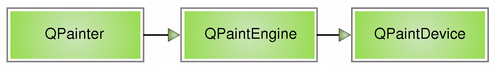
\includegraphics[width=\textwidth,height=!]{img/paintsystem-core.png}
  \caption{Schemat budowy systemu renderowania w bibliotece Qt}
  \label{paintsystem-core}
\end{figure}

\chapter{Określenie problemu i proponowane rozwiązanie}

Przedmiotem pracy jest stworzenie prototypowego serwera hostującego desktopowe aplikacjie oparte o biblioteki Qt oraz KDE. Na żądanie klienta serwer uruchamia wybraną aplikację oraz wstrzykuje kod odpowiedzialny za komunikację klienta z procesem aplikacji i przesyłanie klientowi danych dotyczących wyglądu graficznego interfejsu aplikacji. 

Postawione zadanie w głównej mierze polega na rozwiązaniu trzech podstawowych problemów:
\begin{enumerate}
  \item Komunikacja między klientem a serwerem
  \item Komunikacja między klientem a aplikacją
  \item Uzyskanie informacji o wyglądzie elementów graficznego interfejsu aplikacji
  \item Symulacja interakcji użytkownika z interfejsem aplikacji
\end{enumerate}

\section{Komunikacja między klientem a serwerem}
%Specyfiką problemu jest jego dwuetapowość. W pierwszym etapipe klient inicjuje połączenie jednorazowo wysyłając zapytanie zawierające informacje o aplikacji, którą klient chce uruchomić oraz identyfikatorze klienta. W drugiej kolejności wymagane jest utworzenie kanału komunikacyjnego między klientem a procesem aplikacji. 

Do realizacji tego zadania stworzony został prosty serwer działający w oparciu o protokół HTTP. Jako zasób domyślny udostępnia on listę dostępnych aplikacji, które klient może uruchomić. Lista ta jest w pełni konfigurowalna po stronie serwera. Inicjalizacja połączenia polega na wysłaniu przez klienta nazwy wybranej aplikacji. Serwer po pomyślnej weryfikacji przydziela klientowi unikatowy identyfikator sesji, uruchamia proces aplikacji i wysyła klientowi skrypt w języku JavaScript zajmujący się przetwarzaniem po stronie klienta.

\section{Komunikacja między klientem a aplikacją}
Do rozwiązania tego problemu konieczne jest utworzenie ciągłego kanału komunikacyjnego między klientem a procesem aplikacji, za pomocą którego będzie możliwe przesyłanie informacji o wyglądzie interfejsu aplikacji oraz informowanie aplikacji o zdarzeniach generowanych przez użytkownika po stronie przeglądarki. Jako, że za cel przyjęte zostało założenie o nieingerowaniu bezpośrednio w kod skompilowanych już aplikacji, postawiono na technikę umożliwiającą załadowanie kodu biblioteki dynamicznej do przestrzeni pamięciowej procesu aplikacji tuż przed jego uruchomieniem. Kod ten ma za zadanie utrzymanie połączenia oraz transmisję danych między klientem a aplikacją.

\section{Uzyskanie informacji o wyglądzie elementów graficznego interfejsu aplikacji}
Każdy element graficznego interfejsu aplikacji (QWidget) jest renderowany w momencie odebrania zdarzenia QPaintEvent z kolejki zdarzeń głównego wątku aplikacji. Dzięki temu istnieje łatwy sposób na uzyskanie informacji o tym kiedy oraz ktory element należy przerenderować aby uaktualnić jego wygląd po stronie klienta. Problemem w dalszyb ciągu pozostaje jednak sposób na uzyskanie informacji o samym wyglądzie. 

Proponowane rozwiązanie polega na zaimplementowaniu abstrakcyjnego urządzenia wyjściowego reprezentującego przeglądarkę WWW po stronie klienta (patrz podrozdział \ref{system_rysowania}). Odpowiednio implementując klasy \emph{QPaintEngine} oraz \emph{QPaintDevice} możliwe staje się uzyskanie szczegółowych informacji dotyczących wygądu widget'ów co z kolei umozliwia stworzenie innowacyjnego formatu przesyłanych danych. Zamiast przesyłać bitmapy z wyrenderowanym elementem można wysłać informację o kolorach, punktach, liniach i innych podstawowych elementach, które zostaną narysowane na urządzeniu docelowym jakim po stronie klienta jest przeglądarka WWW z obsługą elementów \emph{canvas}.

\section{Symulacja interakcji użytkownika z interfejsem aplikacji}
Interakcja użytkownika z aplikacją sprowadza się do obsługi następujących zdarzeń:
\begin{enumerate}
  \item Ruch myszy nad elementem
  \item Wciśnięcie, zwolnienie oraz dwuklik przycisku myszy
  \item Zmiana położenia kółka myszy
  \item Wciśnięcie oraz zwolnienie klawiszy na klawiaturze
  \item Zmiana rozmiaru okna aplikacji poprzez przeciąganie jego krawędzi
  \item Zamknięcie, minimalizacja lub maksymalizacja okna aplikacji
\end{enumerate}
Większość z wyżej wymienionych elementów jest obsługiwana jako zdarzenia w języku JavaScript większości dzisiejszych przeglądarek. Proponowane podejście na rozwiązanie tego zagadnienia polega na stworzeniu formatu danych bazując na notacji JSON (JavaScript Object Notation). Dane w tym formacie przesyłane do serwera są następnie poddawane walidacji i konwersji na obiekty zdarzeń biblioteki Qt. Zdarzenia takie są następnie przesyłane do kolejki zdarzeń w głównym wątku aplikacji. 

Odbiorcą zdarzenia jest widget, który wygenerował dane zdarzenie po stronie przeglądarki bazując na hierarchicznej budowie interfejsu użytkownika. Wyjątkami są tutaj zdarzenia klawiatury, które nie mają bezpośredniego odbiorcy w momencie ich zaistnienia. Aplikacja sama decyduje o tym, który element powinien odebrać zdarzenie. Domyślnie jest to widget, który atualnie posiada tzw. focus, a to z kolei zależy od poprzednich zdarzeń oraz logiki samego programu. W celu symulacji podobnego zachowania decyzja o odbiorcy zdarzeń klawiatury podejmowana jest po stronie serwera bazując na aktualnym stanie aplikacji.

\chapter{Implementacja}
Text in first chapter ...



\section{Po stronie serwera}
\label{sec:implementation_server}

\section{Po stronie klienta}

\subsection{Biblioteki pomocniczne}
Podczas pracy z projektem zostały wykorzystane popularne biblioteki ułatwiające podstawowe zadania. Wszystkie z nich są darmowe nawet w wykorzystaniu komercyjnym oraz całkowicie otwarte.
* jQuery
* jQuery-UI
* jQuery-mousewheel
* sylvester.js

\subsection{Połączenie}
Klient po załadowaniu początkowej strony dokonuje połączenia WebSocket z serwerem na port podany na stronie. Następnie nasłuchuje na informacje od serwera i na każdą z nich reaguje. Komunikaty w formacie JSON w drugą stronę wysyłane są po zajściu zdarzeń po stronie klienta, np. ruchu myszą. Dokładny opis zdarzeń znajduję się w sekcji **TODO**

\subsection{Window manager (ang. zarządca okien)}


\subsection{Rysowanie widgetów przy pomocy elementu canvas}


\section{Format danych}

\subsection{Dane wysyłane przez serwera}

\subsection{Dane wysyłane przez klienta}

\section{Napotkane problemy}
\begin{enumerate}
  \item rysowanie za pomocą zdarzeń (konieczność kolejkowania widgetów)
  \item Znikający \emph{focus} okna aplikacji
  \label{problems_focus}
  \item Kody znaków klawiatury
  \label{problems_keyboard}
  \item Łukasz Stanisław więcej problemów nie miał... Kolej na problemy Jana Edwarda
\end{enumerate}

Ad.\ref{problems_focus} Biblioteka Qt stanowi niejako nakładkę dla natywnego zarządcy okien systemu operacyjnego. W zwizku z tym o kolejności okien na stosie decyduje system operacyjny. Qt podejmuje jedynie odpowiednie czynności w celu aktualizacji graficznego interfejsu aplikacji w zależności od aktualnego stanu konkretnych okien definiowanego przez system operacyjny. W sytuacji kiedy użytkownik nie prowadzi żadnej intrakcji z systemem operacyjnym a jedynie z aplikacją, mogło by się zdarzyć, że niektóe zdarzenia było by ignorowane przez aplikację. Przykładem takiej sytuacji jest wprowadzanie tekstu na klawiaturze. Qt przesyła zdarzenia klawiatury do widgeta, który aktualnie posiada focus w oknie, które znajduje się na szczycie stosu okien w systemie operacyjnym. W momencie kiedy dwóch zdalnych użytkowników uruchomiło by aplikację na tym samym serwerze, zdarzenia jednego użytkownika były by ignorowane ponieważ tylko jedno okno jednej aplikacji może być na szczycie stosu. 

Rozwiązaniem tego problemu była reimplementacja odpowiednich metod Qt w celu symulacji zachowania stosu okien systemu operacyjnego wewnątrz samej aplikacji. W rezultacie aplikacja "myśli", że jest aktywna i znajduje się na szczycie stosu okien.

Ad.\ref{problems_keyboard} 
Qt platformowo niezależny opis kodów znaków klawiatury za pomocą zdefiniowanego typu wyliczeniowego \emph{Qt::Key}\footnote{http://doc.qt.digia.com/qt/qt.html\#Key-enum}. Niestety przeglądarki nie są dobrze ustandaryzowane i ich numeracja klawiszy znacznie różni się nie tylko między platformami ale również między różnymi ich wersjami. Dodatkowo przeglądarki często nie wspierają wszystkich klawiszy przez to zakres kodów znaków jest inny niż w przypadku biblioteki Qt.

Powyższe problemy wymusiły konieczność zaimplementowania metody konwertującej po stronie klienta kody klawiszy na odpowiadające im wartości typu wyliczeniowego \emph{Qt::Key}.

\chapter{Testy aplikacji}
Natestowaliśmy się, że hoho

\section{Testy w środowisku lokalnym}
Wszystko spoko.

\section{Testy w sieci Internet}
Nie było jak stestować.

\chapter{Podsumowanie}
Wszystko wyszło gitara. Jesteśmy z siebie dumni. Pozdrawiamy mamę, tatę i dudniącego Krzysztofa.

%+Make Index
\printindex
%-Make Index

\end{document}